\begin{figure} [h]
         \centering
         \caption{ Darstellung der von Gnuplot erzeugten Plots. Ausgewählt wurden zufällig 2 aus 50 durchgeführten Lösungen. Pro Reihe ist jeweils das Ergebnis einer Lösung dargestellt. Auf Basis dieser Plots kann eine Beurteilung der Modellgüte und eine Untersuchung der Einflüsse durch Optimierungsparameter durchgeführt werden. Diese werden in der kommenden Woche durchgeführt. }
%         \label{fig:3}
%         
         \begin{subfigure}[t]{0.34\textwidth}
                 \centering
                 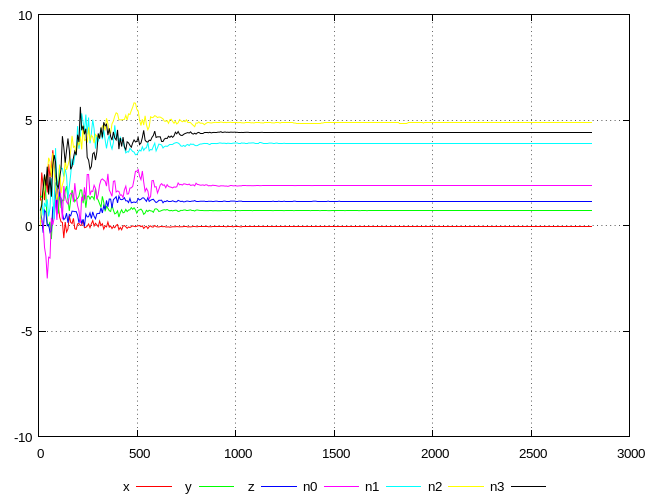
\includegraphics[width=\textwidth]{common/img/objectVar0.png}
                 \label{fig:ResA0}\textit{}
         \end{subfigure}
%         
\qquad
         \begin{subfigure}[t]{0.34\textwidth}
                 \centering
                 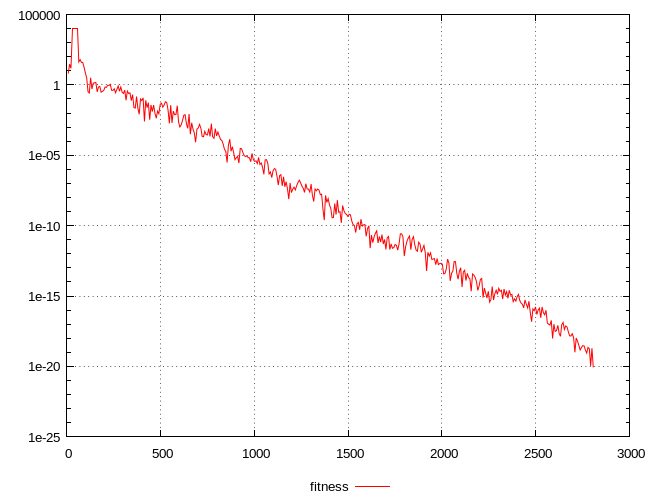
\includegraphics[width=\textwidth]{common/img/fitness0.png}
                 \label{fig:ResB0}
         \end{subfigure}
%
\qquad
         \begin{subfigure}[t]{0.34\textwidth}
                 \centering
                 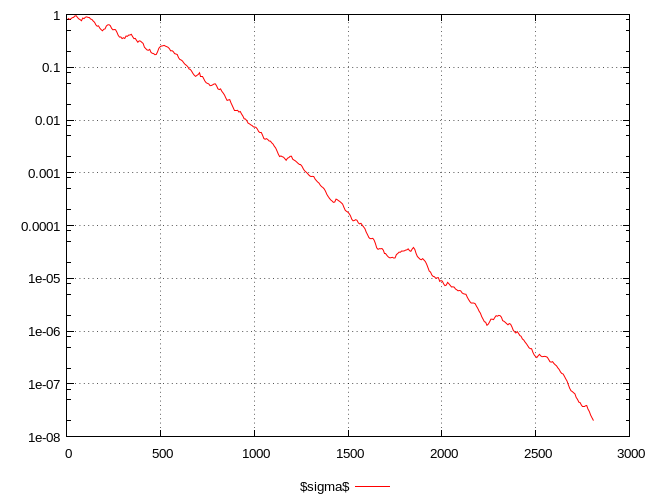
\includegraphics[width=\textwidth]{common/img/sigma0.png}
                 \label{fig:ResC0}
         \end{subfigure}
\\
         \begin{subfigure}[t]{0.34\textwidth}
                 \centering
                 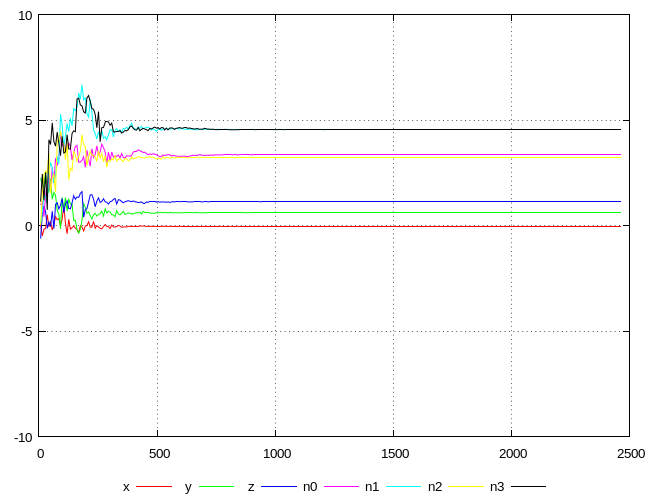
\includegraphics[width=\textwidth]{common/img/objectVar20.png}
%                 \vspace{.1cm}
                 \caption{ Verlauf der optimierten Parameter; Bei diesem Modell wurden 7 freie Parameter optimiert. }
                 \label{fig:ResA20}\textit{}
         \end{subfigure}
%         
\qquad
         \begin{subfigure}[t]{0.34\textwidth}
                 \centering
                 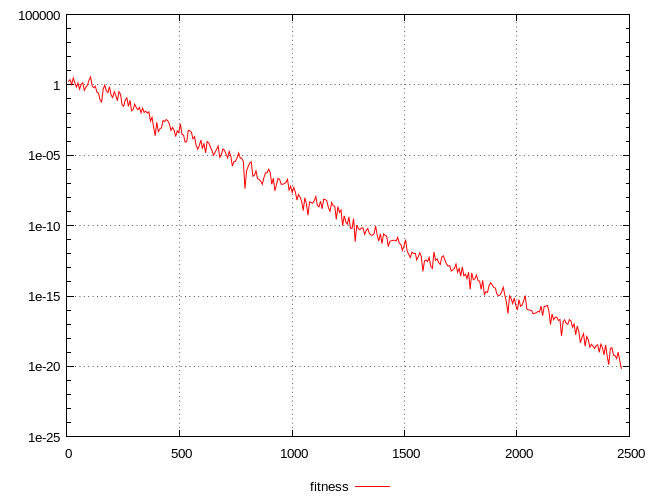
\includegraphics[width=\textwidth]{common/img/fitness20.png}
%                 \vspace{.1cm}
                 \caption{ Verlauf der Fitness der Lösung; Das Abruchkriterium wurde auf $\epsilon<10^-21$ eingestellt }
                 \label{fig:ResB20}
         \end{subfigure}
%
\qquad
         \begin{subfigure}[t]{0.34\textwidth}
                 \centering
                 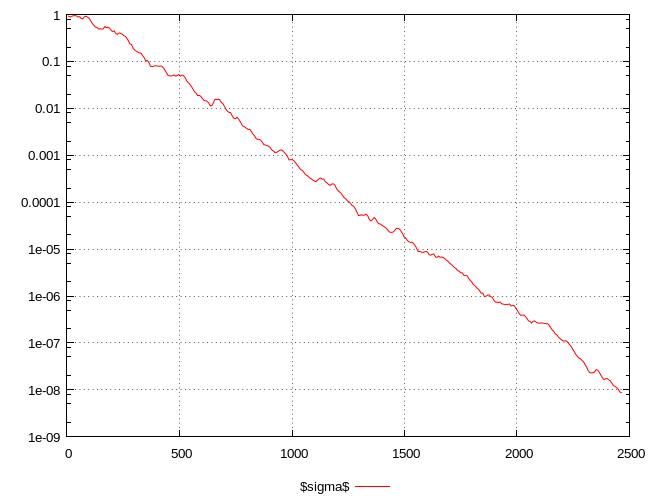
\includegraphics[width=\textwidth]{common/img/sigma20.png}
%                 \vspace{.1cm}
                 \caption{ Verlauf von $\sigma$ während der Lösung; Sigma steuert unmittelbar die Schrittweite des Algorithmus }
                 \label{fig:ResC20}
         \end{subfigure}
\end{figure}